%!TEX root = project.tex

\chapter*{About this project}
\paragraph{Abstract}
The Unity 3D game engine provides a great framework for any novice game developer, even big game studios are using this engine as a bases for their triple A games. Because of the support available, I have chosen to use the Unity 3D engine as the framework for this specific open world 3D game. During the implementation phase, I've found that game development is much more complicated then I previously expected. For instance the assets required to develop a game range immensely, from models, textures, level design, gameplay scripting, player progression, environment to game physics, the amount of work involved seemly never ended. Games today are also quite graphics intensive and require teams of artists, modelers and level designers to create realistic environments for the player to experience and enjoy. 
The original concept of the game was quite simple, it was described to be farming game that required players to buy and sell cattle that will eventually allow the player to grow the farm into a profitable enterprise. The project's artwork, UI interface and storyline developed over time during the implementation stage, which lead me research different areas I've never delved into before and consumed a considerable amount of my time. The game's implementation as I expected proved to be quite challenging, it was an interesting endeavor although Unity's 3D game engine development tools help negate the amount work involved in the project. This paper follows the development of this application and covers in detail about the technologies and software written during the project's progression.

\paragraph{Authors}
The authors of this document; John Walsh, B.Sc. Ordinary Degree - GMIT

\chapter{Introduction}
The 3D gaming world has evolved immensely over the last few years. More gamers are looking to new devices like the mobile platform whether it be an Android and iOS device. This presents new challenges for game develops to not only target multiple platforms, but also deliver a well refined, complex and engaging story lines with high resolution textures and models. This problem is further compounded when developers only have access to limited resources these small devices provide. I'll be going into detail about some of the challenges I faced during design and implementation stages of this mobile 3D game project and finally wrap up the overall product that has been developed and released to the market. Work on this project has been contracted by Pat McNeill at the company Agmanor, via an Enterprise Ireland Voucher.
   
\section{Context}
The game world concept requires the player area to be constructed in 3D open environment, which means the player will be able to freely navigate their way around the virtual world. A joystick type control has been implemented to allow users with touchscreen features on their devices to control the character. Camera view angles will be primarily locked into an isometric angle giving the user a third person view of the character. From this point of view, the player will be able to see most of the environment and intractable game objects around the character. Player's interact with the game's menu system primarily by touch. Frameworks like NGUI [~\cite{NGUI}] have been employed to help scale and display the menu's elements in a consistent design, which is important when dealing with varying screen sizes. Transitions between levels will be handled when the player’s character comes into contact with a special object / area in-game that triggers an event to display a menu, which in turn allows the player move from one level to another. 
Target audiences for this game could roughly range from 6 + or older, I'm not entirely certain what age group this game fits into. I believe the game has potential to grow and develop into more than farming simulator game, for instance from an education point of view, the game could be modified to teach kids more about farm animals and how to properly look after animals.
Once the game has been fully implemented, the application will be released to the market, as of writing I plan to launch the games on both Android and iOS platforms.  

\section{Objectives}
The first objective of the project was to design an application that would satisfy both the client and gamers alike when fully implemented and released to the market. During initial few weeks of development, I had to up skill on the different tools available in the Unity IDE editor. The 3D landscape view of the world was bare and dull in the beginning, everything would either needed to be developed by myself or sourced by third party assets developers. The Unity store contained plenty of pre-made models and texture that could be easily modified and adapted into the game.
Since this game primarily evolves around having an open environment for the player to explore, tools like the 3D terrain editor and animation engine were experimented with considerably during the initial versions of the game. 
After some time getting acquainted with the development tools, it was at this stage I needed to source proper assets that would fit with the theme, artwork and gameplay features. The developers of Unity 3D have constructed an assets store that contains some useful materials and tools that greatly decrease the development time required to construct scene levels and game objects.
\section{Chapters Review}
In this chapter I'll be briefly reviewing the different areas of this paper. From the design and planning phase to the implementation phase.
\subsection{Methodology}
In this chapter I'll cover the different development tools and practices I've used during the implementation phase of the project. Work on the project has been recorded and documented using the tool collaboration GitHub, I believe it would be prudent to review commits in project repository.
\begin{itemize}
	\item Provide a context for your project.
	\item Set out the objectives of the project
	\item Briefly list each chapter / section and provide a 1-2 line description of what each section contains.
	\item List the resource URL (GitHub address) for the project and provide a brief list of the main elements at the URL.
\end{itemize}

\subsection{Technology Review}
The different technologies used to design and implement the project from start to finish. Everything from the tools used to the software development approaches employed to create an efficient and effective foundation for the game to be built upon.
\subsection{System Design}
System design will cover the different modules and classes implemented to perform a particular function whether it be gameplay scripting to UI implementation.
\subsection{System Evaluation}
The analysis of game performance and behavior of system components when new items or features are added to the game. Details of changes during the implementation stage of development and if they effected other components of gameplay, UI or other areas of the game's system.
\subsection{Conclusion}
Final conclusion from the overall design and development of the project, I will review the final product and discuss different parts of the implementation that could've been developed differently, maybe even more efficiently then the current version of the project.
\section{Resources}

\chapter{Methodology}
About one to two pages.
Describe the way you went about your project:
\begin{itemize}
\item Agile / incremental and iterative approach to development. Planning, meetings.
\item What about validation and testing? Junit or some other framework.
\item If team based, did you use GitHub during the development process.
\item Selection criteria for algorithms, languages, platforms and technolo-gies.
\end{itemize}

\chapter{Technology Review}
In the world of games development, especially in mobile games, Unity 3D has a great SDK in which developers can design, create and implement their ideas into working games across multiple platforms [~\cite{Unity3D}]. When game developers want to create games, they normally avoid the use of native application completely. The libraries in Android and iOS aren't game oriented, platform designers mainly focus on providing useful APIs for general usage of the phone's capabilities, not generate 3D interactive worlds. So usually when a game designer looks for good foundation to develop his or her game, they may choose something like Unity3D. This framework provides a good bases for developers to target many different platforms including popular living room consoles like the PS4 and Xbox One. Mobile targeted games need to deal with unique problems, "many critical issues and presents some considerable challenges for games developers, such as the typical resource constraints" [~\cite{RAD-Game-Development}]. The issues raised in this paper highlight the problems developers should be aware of when developing for mobile platforms. The available resources on devices varies greatly, which can restrict the amount of content, features and overall gameplay. I've been working on a 3D mobile game based in Unity that targets the Android platform. I've experienced the same resource problems in my game, especially with older mobile phones. Normally it’s caused by shadow and partial effects that can severely drop the frame rates of the game. Unity allows the developer to target a specific API level in Android, for example if you target version 2.3 which is codenamed 'Gingerbread', all Android versions 2.3 and above could in theory run the game. What I mean by 'potentially' its means that the game may run on the device if enough resources like video memory and CPU processing power is available. Referring back to the paper 'Rapid Mobile Game Development', the issues of resource management and game portability were raised. They stated that "Unity does not require much effort to work with multiple platforms", I believe that porting a game to another platform could be a challenging task, for instance some platforms require different types of input, an example would be from a keyboard and mouse or a joypad on a games console, The task of porting a game that utilizes the accelerometer or gyroscope in a mobile device would also increase the difficulty of task, nearly requiring the game to be completely re-designed. Many alternatives exist over the Unity framework in the mobile game development, probably too many to go into detail, but one that has peaked my interest is the Unreal Engine [~\cite{Unreal-Engine}]. This game engine pushes the boundaries of the latest hardware available in the mobile gaming world, for example the newest Nvidia’s Tegra K1 mobile GPU processor has 192 cores that can fully utilize the latest multimedia APIs like DirectX 11 and OpenGL 4.4 [~\cite{Nvidia-K1}]. This means the latest games usually found only on the PC, Xbox and PlayStation can be ported to a mobile platform which makes the Unreal Engine framework an ideal choice for a professional gaming studio to utilize. The same architecture used in the K1 can be found in the latest PC graphics hardware today, which is usually found in powerful gaming PCs and fast GPU based supercomputers. Unity reduces this problem by optimizing each platform it can target making it truly a great framework to develop, create and bring your ideas to life.
\subsection{The Editor}
Unity's editor is quite intuitive and flexible IDE allowing you to customize the overall layout, which is extremely useful when you have multiple monitor setup. Unity work flow is fast and interactive within scene and game view ports. Three dimensional environments can easily be created once your comfortable with project hierarchy and asset import system, simply drag and drop your assets into the scene to get level populated. One feature I've found quite useful is the re-usable prefab system. This system allows developers to reuse models and textures to create completely new and original looking game objects. Assets can either be sourced directly from the unity store or if you have your own game object creations ready to go from modeling applications like Blender, Autodesk or Sculptris for example. These modeling applications have great support within Unity rendering engine. As of writing, Unity can read .FBX, .dae (Collada), .3DS, .dxf and .obj modeling files [~\cite{Unity-Models-Support}]. Unity also a number of handy tools like the terrain editor, which allows developer create detailed and vibrate looking environments. The physics engine ties directly into the terrain plane, following each bump and curve the tools create to allow game objects like the player's character and animals to walk upon. Each game object in the scene has a component called the 'Transform' position, this ability allows game objects store the rotation, scale and parenting state independently from one another. 

\begin{figure}[!ht]
	\caption{The Scene Transform Position}
	\centering
	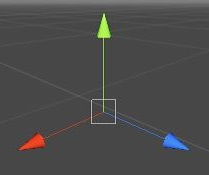
\includegraphics{img/transform.jpg}
\end{figure}

\subsection{World Environment}
The terrain editor also allows you to place foliage around the environment, trees, plants, grass and shrubs for example can be placed in great numbers relatively quick and efficiently. However, the amount of resources required steadily increases as more objects are placed into the scene, I've had monitor the amount of draw calls required to run the scene. For instance; an object with one material equals a single draw call but an game object with four materials equals four draw calls. The GPU on a device would receive a 'hit' for every draw call requested, less draw calls means better performance equaling more fps at runtime.
\subsection{Game Objects}
On the topic of game objects, scripts written in either C-Sharp or JavaScript can at runtime instantiate game objects. For instance, I've used such scripts to spawn the player's animals in specific areas with vegetation. To give the animations from each of these animals some realistic purpose, the animation state engine allows the developer specify which animations play at certain times, for instance if theres vegetation object detected using a collision trigger component, a state machine variable could be set, thus allowing the animation engine known when to play the correct animations. For this project, I've used the very same methods to allow the player's character notify the animation engine when input from the virtual joystick is detected. The player controller script can independently control the speed of a specific animation, depending on the level of movement requested by the player. Input can is taken from 'Virtual Axes', by default the Unity editor maps these axes in the 'Horizontal' and 'Vertical' planes to w, a, s, d and the arrow keys, this is usually more suitable to conventional games like FPS shooters. I've modified the controls found in the input manager to reverse the axes coming from both planes to suit the virtual controls suite.
\subsection{Lighting}
Another important aspect of game development is lighting, within the unity editor you have a number of option available to you when developers want to achieve a specific mood or lighting effect to give the player's a more realistic setting to the environment. Scene textures and models can be greatly effected when lighting effects like flares, spot lights and bounce reflections really making the game come to life when applied correctly. For instance the following images taken from the Unity's docs web page shows how influential light can be to the environment.

\begin{figure}[!ht]
	\caption{Mood Lighting 1}
	\centering
	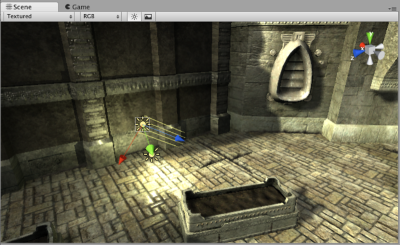
\includegraphics{img/light-mood-1.png}
\end{figure}

You can see how bright areas lit from the lighting components are, and how dark shadows are in contrast. Lighting is all about setting the correct mood for players to experience. Take the next figure, it's comprised of the exactly same scene with only the intensity and color of the lighting component being modified.

\begin{figure}[!ht]
	\caption{Mood Lighting 2}
	\centering
	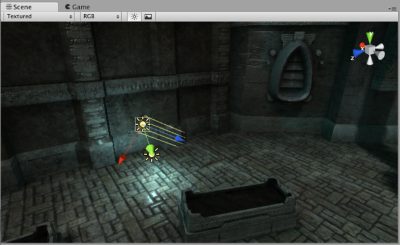
\includegraphics{img/light-mood-2.png}
\end{figure}

Lighting as you can see plays a major role in game development, for my own project I've applied only basic lighting techniques to the area of play because performance issues would incur and reduce the frame rate. Shadows have also been reduced quite considerably because of performance issues. As I stated before mobile device rarely have enough resource to run with full shadows and lighting effects like flares, HDR or highly detailed shading.
\subsection{Rendering Detail}
The level of detail rendered on screen can be adjusted to suit the platform your targeting. The LOD or 'Level of Detail' from objects can vary depending on the main camera adjustment, for example if you set the view distance fairly low the render detail of objects in the game scene will change depending on how far the main camera is position away from a specific game object. There exist a number of different levels, ranging from 'LOD 0' which is stated to display the highest level of detail to 'LOD 1' and 'LOD 2', which are the lowest level of rendering. Developers can balance between these levels to find an acceptable level for the specific platform their targeting, especially when porting to mobile platforms with limited resources.

\subsection{Physics}
Having convincing 3D physical behaviour is essential when creating a open world game. Game objects must have certain components to correctly accelerate, collied and react against other world objects. With just a few parameter settings you can easily simulate virtual objects just like the real thing, depending on what your creating of course. Objects can be further manipulated using scripts written in either C-Sharp or JavaScript. For example if you wanted and object to be behave like if it were in low gravity environment and bounce around like a rubber ball its quite simple as attaching a physics behaviour script to the object. 

\subsection{Scripting}
Unity's scripting system is quite powerful, each game object usually has many different components with various responsibilities, for example rigidbodies, box colliders and hinge joints for physics simulation. These components can be influenced by scripts attached to the game object, for example if I wanted to move the game object all I would need to is access the transform component using the following snippet.

\begin{minted}{csharp}
public class UsingOtherComponents : MonoBehaviour
{
	public GameObject otherGameObject;
	
	private AnotherScript anotherScript;
	private YetAnotherScript yetAnotherScript;
	private BoxCollider boxCol;
	
	void Awake ()
	{
	  anotherScript = GetComponent<AnotherScript>();
	  yetAnotherScript = otherGameObject.GetComponent<YetAnotherScript>();
	  boxCol = otherGameObject.GetComponent<BoxCollider>();
	}
}
\end{minted}

Unity supports two different languages natively, C-Sharp and a JavaScript like language they call UnityScript. The .NET framework provides a powerful, stable and dependable foundation to your project's script writing. I believe is far easier to use an object orientated language for game development projects like the one I'm undertaking, as sections of project can be split among teams of programmers. 
The JavaScript like language is other option when implementing your game control logic, I would argue against using this language because in the long term adding new features and maintaining the source would become quite difficult as the complexity and size of the overall project expands.

\subsection{Audio}
The audio system in Unity gives the developer complete control over how sounds are emitted by objects and heard by listeners. A game object with a sound component can attach a sound file to itself and play it with a degree of intensity and volume level. These sounds are picked up by 'Listener' components, which are usually attached to player controlled game objects. Sound can be emitted from audio sources either in a 2D or 3D form. Sound emitted in the 2D form is not usually used in 3D games as the sound has no distance fade control like 3D emitted sound contains. The fade distances are quite useful in simulating realistic ambient sounds effects.
I’ve sourced a lot of sound effects from various places, all royalty free of course. To name a few sources, 'SoundCloud', 'FreeSound' and other various content providers on the Unity assets store.

\subsection{User Interface}
http://docs.unity3d.com/Manual/UICanvas.html

\begin{itemize}
\item Describe each of the technologies you used at a conceptual level. Standards, Database Model (e.g. MongoDB, CouchDB), XMl, WSDL, JSON, JAXP.
\item Use references (IEEE format, e.g. [1]), Books, Papers, URLs (timestamp) – sources should be authoritative. 
\end{itemize}

\section{C-Sharp Language}
The Unity game engine utilizes the C-Sharp programming language. Backed by the latest .NET 4.6 framework, developers can take full advantage of the powerful and stable underlining libraries. 

The following sample is from the game controller class, which allows the player data to be saved using serialization. 

Saving the Player's Data to File
\begin{minted}{csharp}
try
{
	FileStream file;
	BinaryFormatter bf = new BinaryFormatter();
	
	// Save player data
	file = File.Open(Application.persistentDataPath + 
		"/player.dat", FileMode.OpenOrCreate);
	bf.Serialize(file, _instance.player);
	file.Close();
	
	// Save cow data
	file = File.Open(Application.persistentDataPath + 
		"/cows.dat", FileMode.OpenOrCreate);
	bf.Serialize(file, _instance.cows);
	file.Close();
	
	Debug.Log ("Saving!");
}
catch (UnityException e)
{
	Debug.Log("Saving Failed! - " + e);
}
\end{minted}

\chapter{System Design}
In this section of the document I'll cover the overall design and implementation of the game with help from UML diagrams to visualize the structure. Throughout this project I've had an object orientated design in mind, but in some cases I've done away with normal design principles for certain areas of the project. Unity's component structure requires scripts to be written slightly different to the normal compose and delegate structure of traditional OO program design ideas. Unity's developers encourage use of the 'GetComponent' method of acquiring new instances of objects and scripts. Because of this variables inside of scripts usually will contain many 'public' access type variables and objects instances.
\subsection{Game Controller Design}
The game controller class is quite an important area in the software design structure. It handles most of the main game control variables and object instances that are used throughout the software class structure. Another important class called 'CheckGC' basically checks at run if an instance of the game controller is present and valid, if no instance is found for some reason then one is created. The game itself can simply not function without one instantiated.

\begin{figure}[!ht]
	\caption{UML Diagram GC}
	\centering
	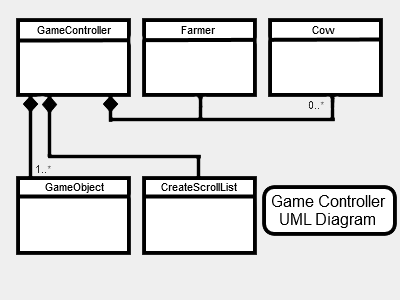
\includegraphics{img/gc_uml.png}
\end{figure}

As you can see I've included the different connections or relationships between these classes. The 'GameController' class fully composes each class found in the design image structure. Classes dependent on the variables inside of the 'GameController', access them through the use of a single static instance called 'instance' and will have it's variable 'set' parameter initialized to private. This will prevent outside classes from mishandling the variable and screwing up the game instance.
\subsection{Animal Controller Design}
Animals in the game require some form of behaviour and movement. The following UML diagram shows the basic aggregation relationship between the 'Cow' and 'CowController' classes. All of the animation and movement logic is contained within the 'CowController' class, also a simple state machine can be found in this class, because each cow object thats instantiated is essentially given its own thread and freedom in the game world. This state machine basically allows the individual animals in game to move and play specific animations when required too.

\begin{figure}[!ht]
	\caption{UML Diagram CC}
	\centering
	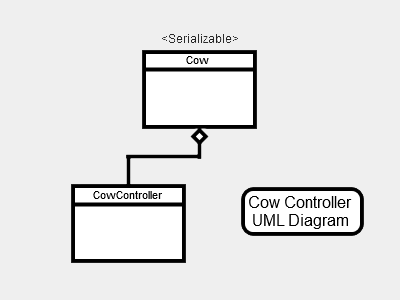
\includegraphics{img/cow_uml.png}
\end{figure}

The controller class also contains logic for a simple enough path finding algorithm that utilizes a Unity component called 'Raycasts' to detect objects around itself to avoid them and continue to a specific coordinate in the game world. I'm not sure if this really classifies as 'AI', but however the game animal object does attempt to seek the shortest path to the location specified. If the animal fails to find a route to the specific location it re-traces its steps to find another route.
This class also contains some control logic for the UI interface to display the correct information to the player when selected. This logic also controls the main camera view and translate it's position smoothly from one point to another without any glitching or laggy movement.

\chapter{System Evaluation}
Testing is probably the most important task of any software project, without testing, programmers could introduce more bugs into the application when fixing or maintaining sections of the source code. It's important to testing each section of application before signing off and releasing a new version of the program. Usually some form of automated testing is written to handle different classes and their subroutines to make sure nothing gets effected from the latest changes in the program. Unit testing is one such form that allows developers continually test as they work. The project I'm currently working does support unit testing, so long as I keep C-Sharp as my main scripting language.
\subsection{Optimizing Graphics Performance}
Optimizing a game for the mobile platform is important task for an game developer, especially when dealing with the problem of limited resources.
Unity has a number of different tools available to diagnose bottlenecks and frame rate problems. The Unity 'Profiler Window' allows you see exactly whats using resources. It also displays how many draw calls are being requested for the GPU and how many CPU cycles required to the run various areas of your game like collision detection, object physics and other CPU intensive calculations. I've used this tool to monitor the amount of resources over the project's development, interestingly enough Unity handles optimizations quite well, I've read that the render engine bundles similar textures into single draw calls reducing the load on a GPU. Even though I'm using relatively basic textures and models in my game, I still worry about frame rate problems, because every new object added to the game scene reduces the performance levels, I aim to target as many mobile devices as possible. The profiler displays data from the game in a timeline, and allows you to see which frames spike. The spikes signify an area of interest you need look into and inspect. The specific frames in these spikes areas in the graph need to be analyzed and debugged to see what component of the game is bottlenecking the application.
\subsection{Testing Hardware}
Mobile hardware ranges quite a lot when you starting talking about all the different generations of iPhones and Android devices that released to the consumer market of the past few years. While the Unity game engine allows you to port too many different platforms like PlayStation and Xbox, I’ve been focusing my attention on the Android platform. This platform can present game development with a couple of problems, one would be the API level. Over the years different versions of Android all the way from 1.5 to 6.0 presents one major problem to the developer. What API level do I develop for?, Unity thankfully handles this problem by allowing the developer to choose the lowest API level required to run the game.
Development hardware consisted of my own personal collection of Android devices, in all different screen sizes and API level versions. It’s quite simple to enable debugging on Android smartphones and tablet devices, the following method usually only applies to later models. Running an unsigned compiled APK file requires you to unlock the phone into developer mode, go into settings and navigate to the section 'About' and from there you should see an option for 'Software Information' or something similar, then 'More' if available and finally hit 'Build Number' seven times. Before I can build project and compile the source into APK file, I first must set or create the “keystore” file. Read more about the file here. It’s basically signing certificate that must be included with project when submitting applications to the Google play store. Also any incremental updates that proceed must also include this special file when building the project before submitting to the store.

\chapter{Conclusion}
Throughout this project I've learned quite a lot about game development, to only not brain storm ideas of gameplay but to implement it into a real project. I'll admit that the game is still its early stages of development and does not provide any sort of solid storyline or dialog, it mainly gives you the general idea of what the game is about. During its development stages I was grasping the tools and features available in Unity, if I were to restart the project tomorrow I would probably go about designing and implementing the game with a completely different method and approach.

During the implementation stage of the project I've learned a great deal about the Unity SDK. Everything from the lighting systems to audio components, game development within Unity quite enjoyable experience. With its simple drag and drop features, level creation and environment setup time is reduced considerably allowing developers to quickly prototype ideas and gameplay features.

Debugging in Unity is difficult to perform, especially when trying to figure out frame rate and performance issues. The included software IDE is a bit crude and flaky at times but it does perform tasks such as line breaking and remote debugging quite well without issue. 

\begin{itemize}
\item Briefly summarize your context and objectives (a few lines).
\item Highlight your findings from the evaluation section / chapter and any opportunities identified.
\end{itemize}

